\documentclass[a4paper,12pot]{article}
\usepackage[polish]{babel}
\usepackage[OT4]{fontenc}
\usepackage[utf8]{inputenc}
\usepackage{graphicx}
\usepackage{listings}
\title{Sprawozdanie kolokwium}
\author{Kamil Bouhaouli}
\date{\today}
\begin{document}
\maketitle
\section{ZAD 1}
\begin{verbatim}
ssh-keygen -f ~/ecdsa-key -t ecdsa -b 521. -> generowanie klucza
ssh-copy-id -i  ~/ecdsa-key mpyzik@pwi.ii.uni.wroc.pl -> kopiowanie klucza na serwer
ssh-add ~/ecdsa-key -> dodanie klucza do klienta
ssh mpyzik@pwi.ii.uni.wroc.pl -> polaczenie sie do serwera z uzyciem klucza
\end{verbatim}
\section{ZAD 2}
\begin{figure}[!htb]
\centering
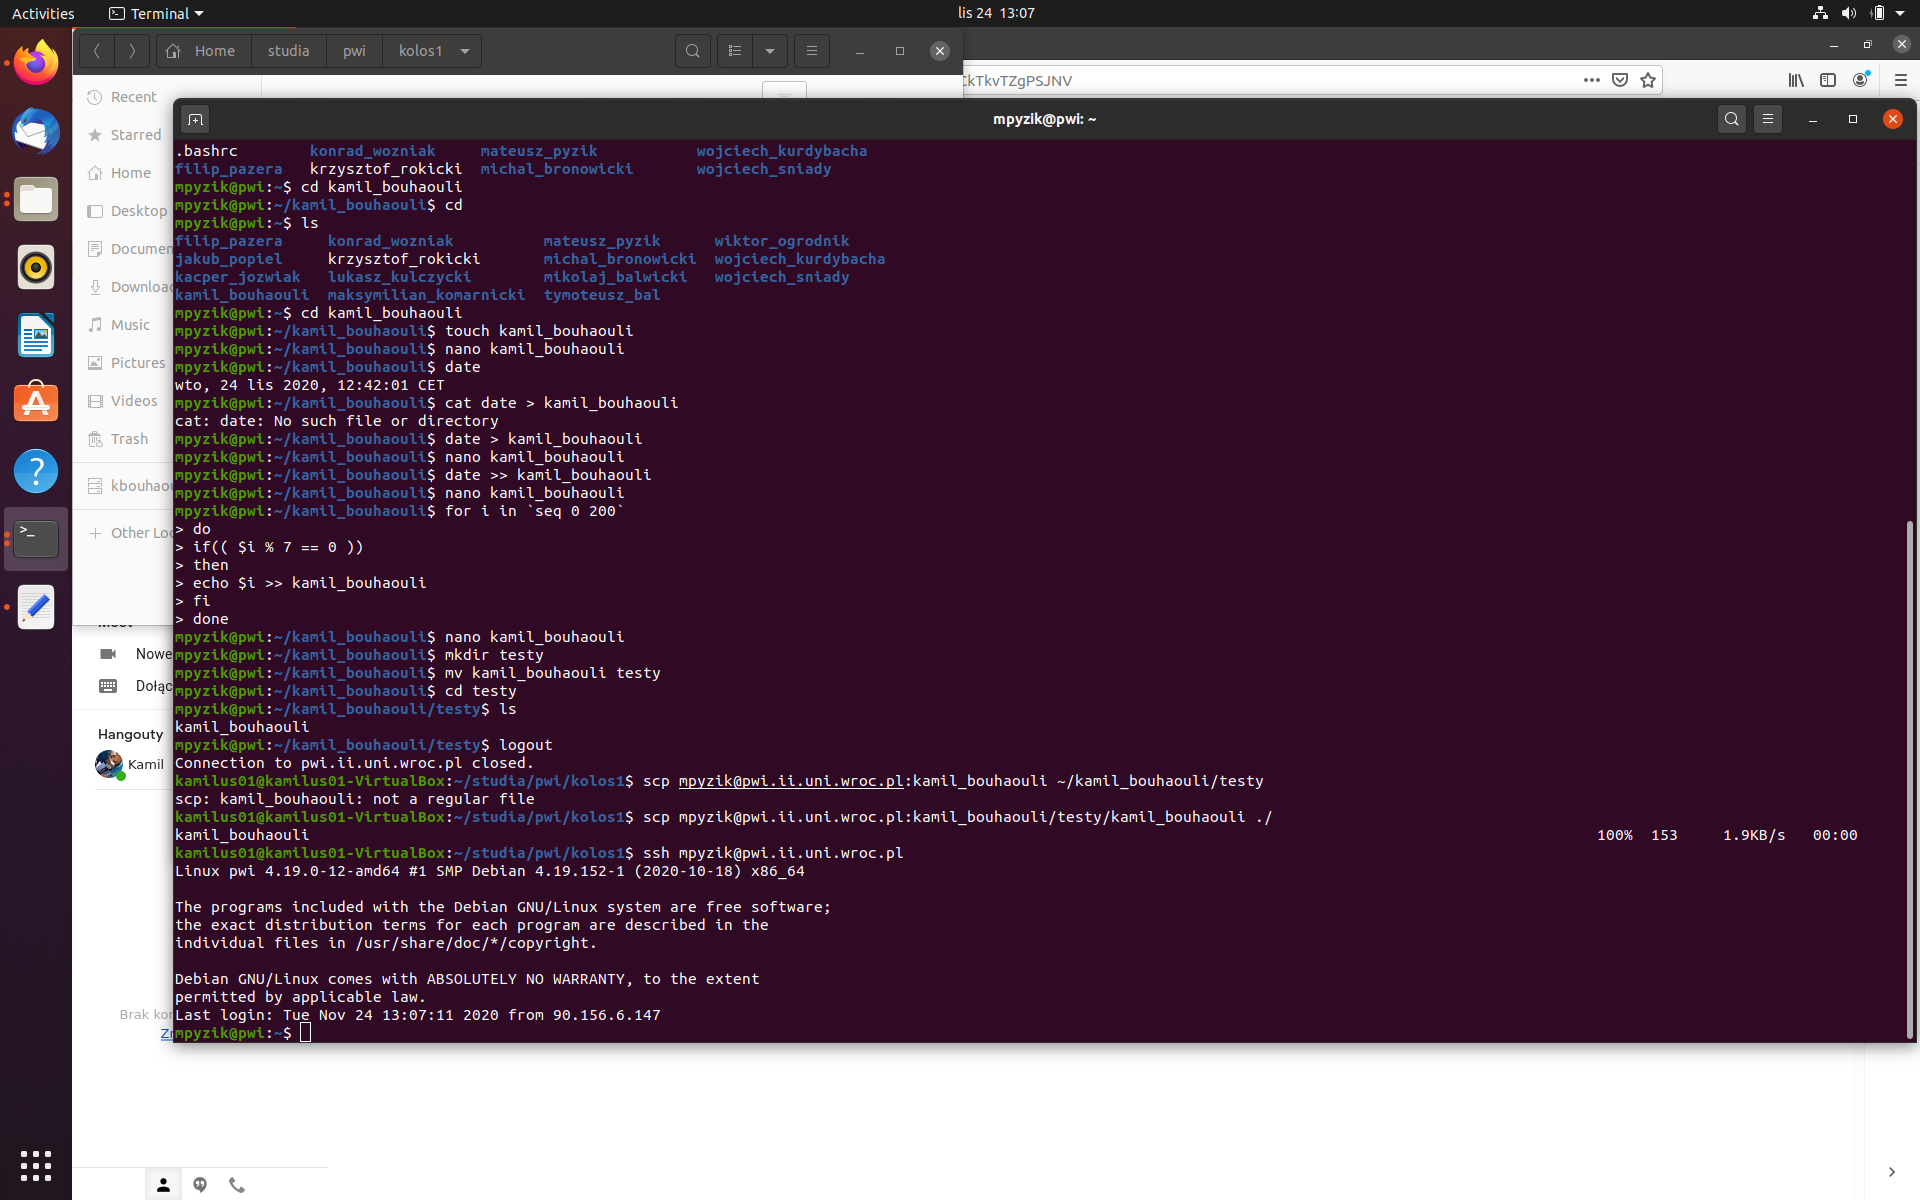
\includegraphics[scale=.25]{s2.png}
\caption{ZAD 2 polecenia uzyte}
\label{fig1}
\end{figure}
\section{ZAD 3}
\begin{verbatim}
for i in `seq 0 4`
do
touch $1.txt
echo `hexdump /dev/urandom | head` > $i.txt
done 

-> Powyzszy kod tworzy pliki 0-4.txt 
i zapisuje do nich wyjscie komendy hexdump /dev/urandom | head

cat 0.txt 1.txt 2.txt 3.txt 4.txt > concat

-> skleja pliki do pliku concat

grep -E "^0.*([a-z0-9][a-z0-9]){4}$" concat > output

-> funkcja sprawdzza czy linijka zaczyna sie od 0 (^0) 
i sprawdza czy ostatnie 4 znaki ({4}$) sa w formacie dwoch powtorzen
 dwoch takich samych podwojnych ciagow znakow obok siebie 
 (([a-z0-9][a-z0-9]){4}$) == 4 ostatnie znaki sa w formacie
   dwoch takich samych dwuznakowych ciagow
  
wc concat 

-> 5 linijek

wc output

-> 0 linijek
\end{verbatim}
\end{document}
